\documentclass[11pt]{article}
\usepackage{hyperref, graphicx, float} 
\graphicspath{{./pics/}}
% Title Page
\title{Assignment 1 - MPP: Message-Passing Programming}
\author{Marian Daogaru, 25685252}
\date{09/05/2017}
\usepackage{geometry}

\geometry{a4paper,
	total={170mm,257mm},
	left=20mm,
	top=20mm,}

\usepackage{fancyhdr}
\pagestyle{fancy}
\fancyhf{}
\rhead{Marian Daogaru, 25685252}
\lhead{FEEG6003}
\cfoot{\thepage}

\usepackage{listings}
\usepackage{color}
\definecolor{dkgreen}{rgb}{0,0.6,0}
\definecolor{gray}{rgb}{0.5,0.5,0.5}
\definecolor{mauve}{rgb}{0.58,0,0.82}
\lstset{frame=tb,
	language=C,
	aboveskip=3mm,
	belowskip=3mm,
	showstringspaces=false,
	columns=flexible,
	basicstyle={\small\ttfamily},
	numbers=none,
	numberstyle=\tiny\color{gray},
	keywordstyle=\ttfamily\color{blue},
	commentstyle=\color{dkgreen},
	stringstyle=\color{mauve},
	breaklines=true,
	breakatwhitespace=true,
	tabsize=3
}

\begin{document}
	
	\maketitle
	\pagebreak
	\tableofcontents
	\pagebreak
	
	
	\begin{figure}[H]	
		\centering
		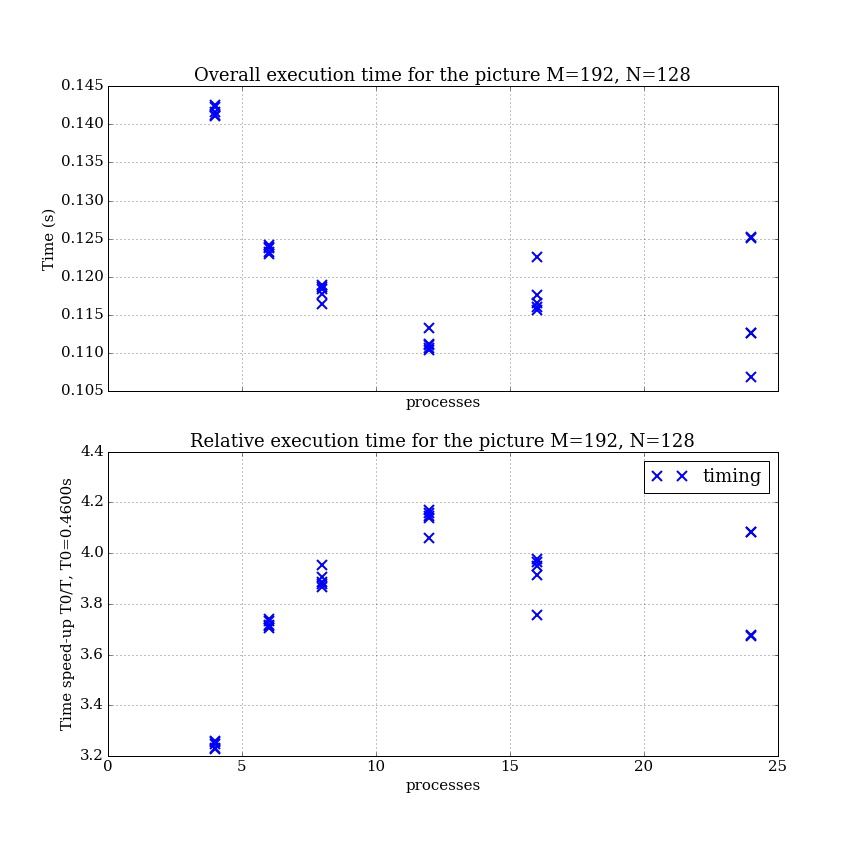
\includegraphics[scale=0.4]{exec_192x128.jpeg}
		\caption{Execution time and relative(to serial) execution time for the 192x128 pixel image.}\label{exec_1}
	\end{figure}

	\begin{figure}[H]	
		\centering
		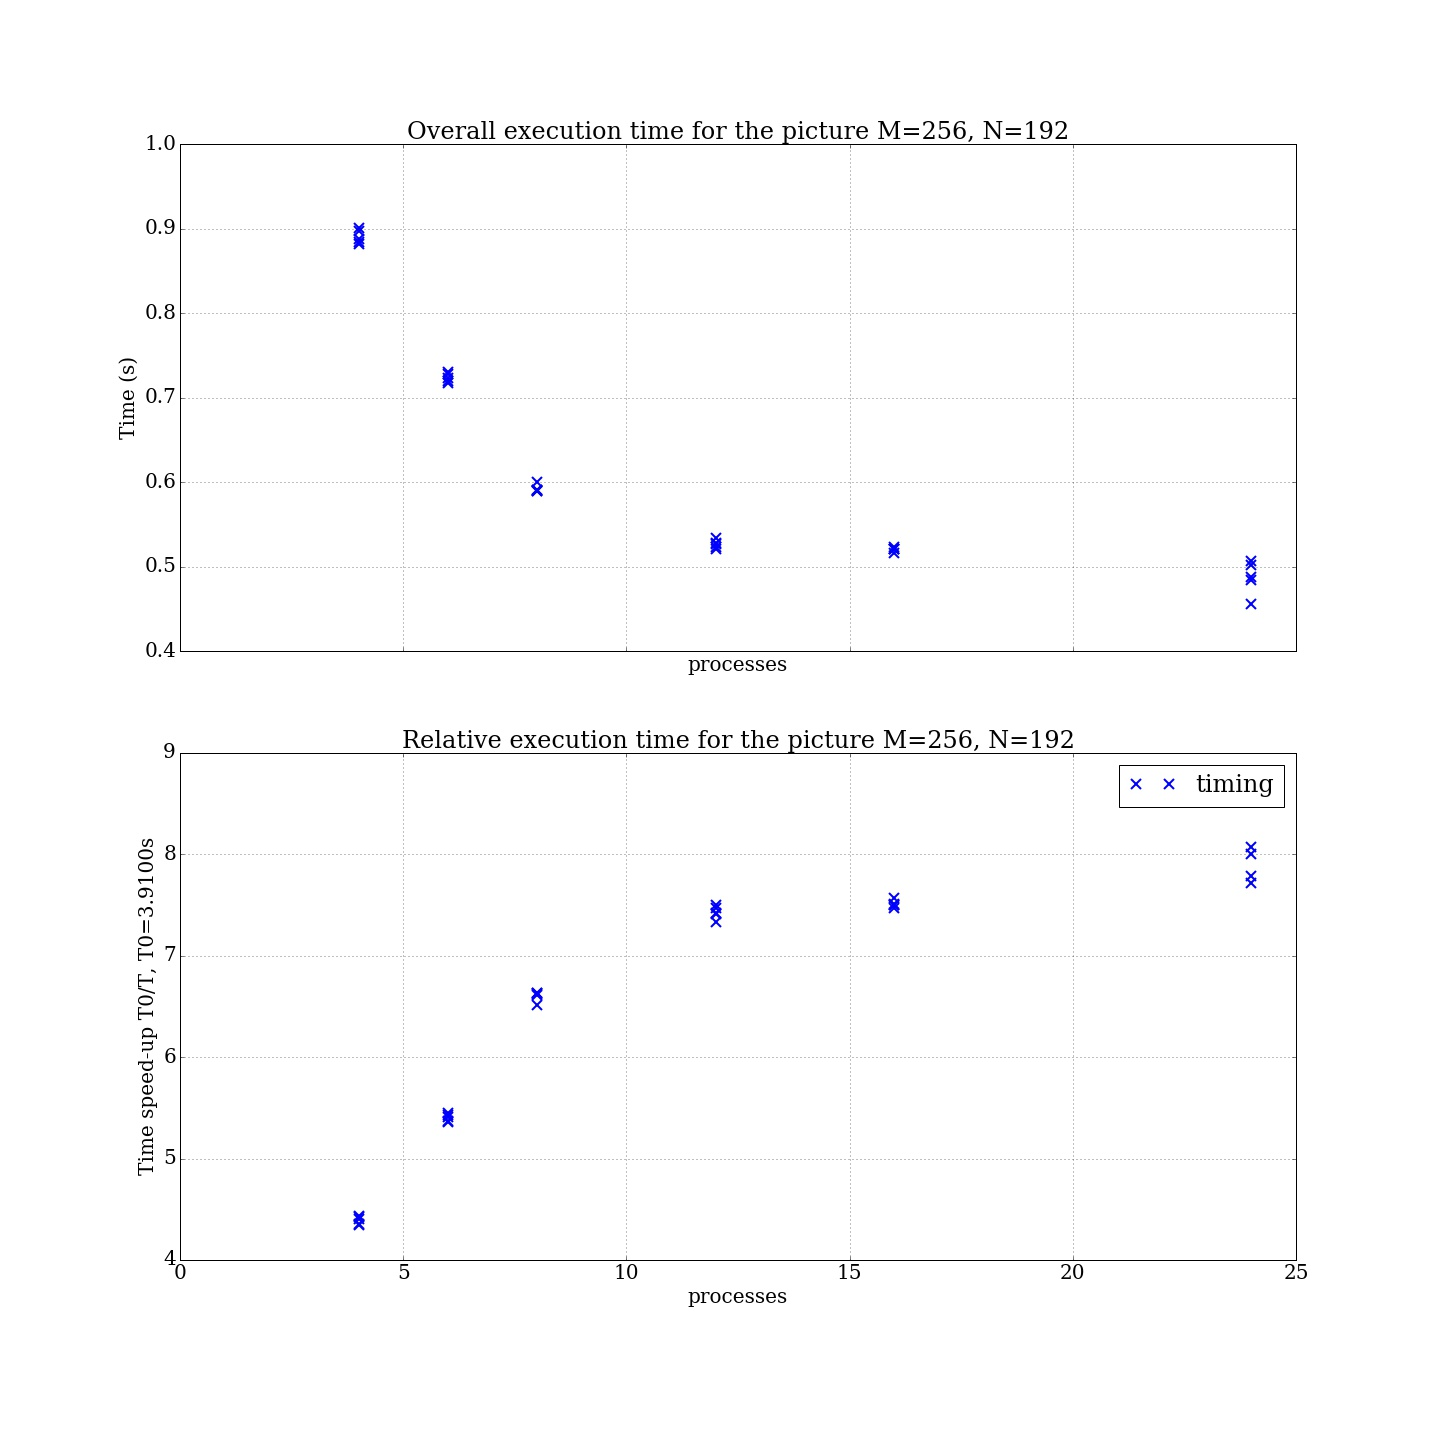
\includegraphics[scale=0.4]{exec_256x192.jpeg}
		\caption{Execution time and relative(to serial) execution time for the 256x192 pixel image.}\label{exec_2}
	\end{figure}

	\begin{figure}[H]	
		\centering
		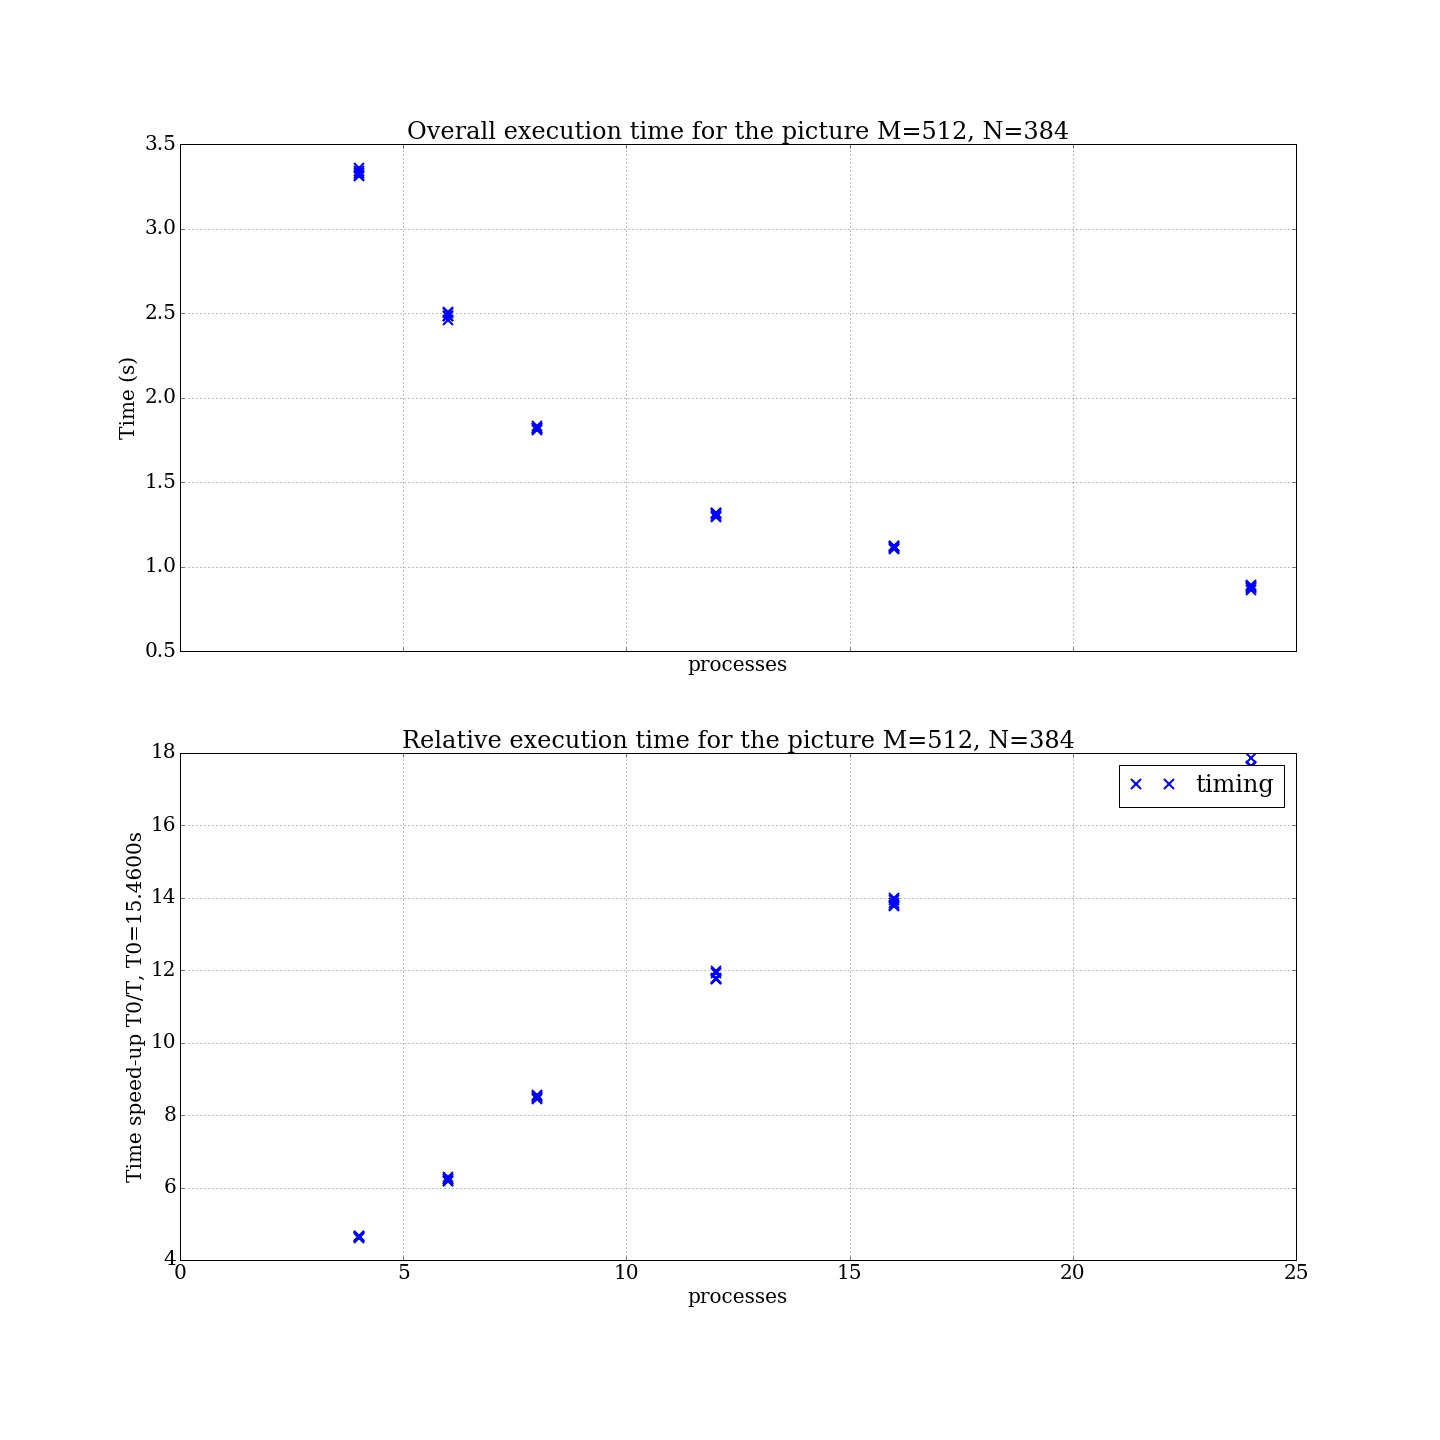
\includegraphics[scale=0.4]{exec_512x384.jpeg}
		\caption{Execution time and relative(to serial) execution time for the 512x384 pixel image.}\label{exec_3}
	\end{figure}

	\begin{figure}[H]	
		\centering
		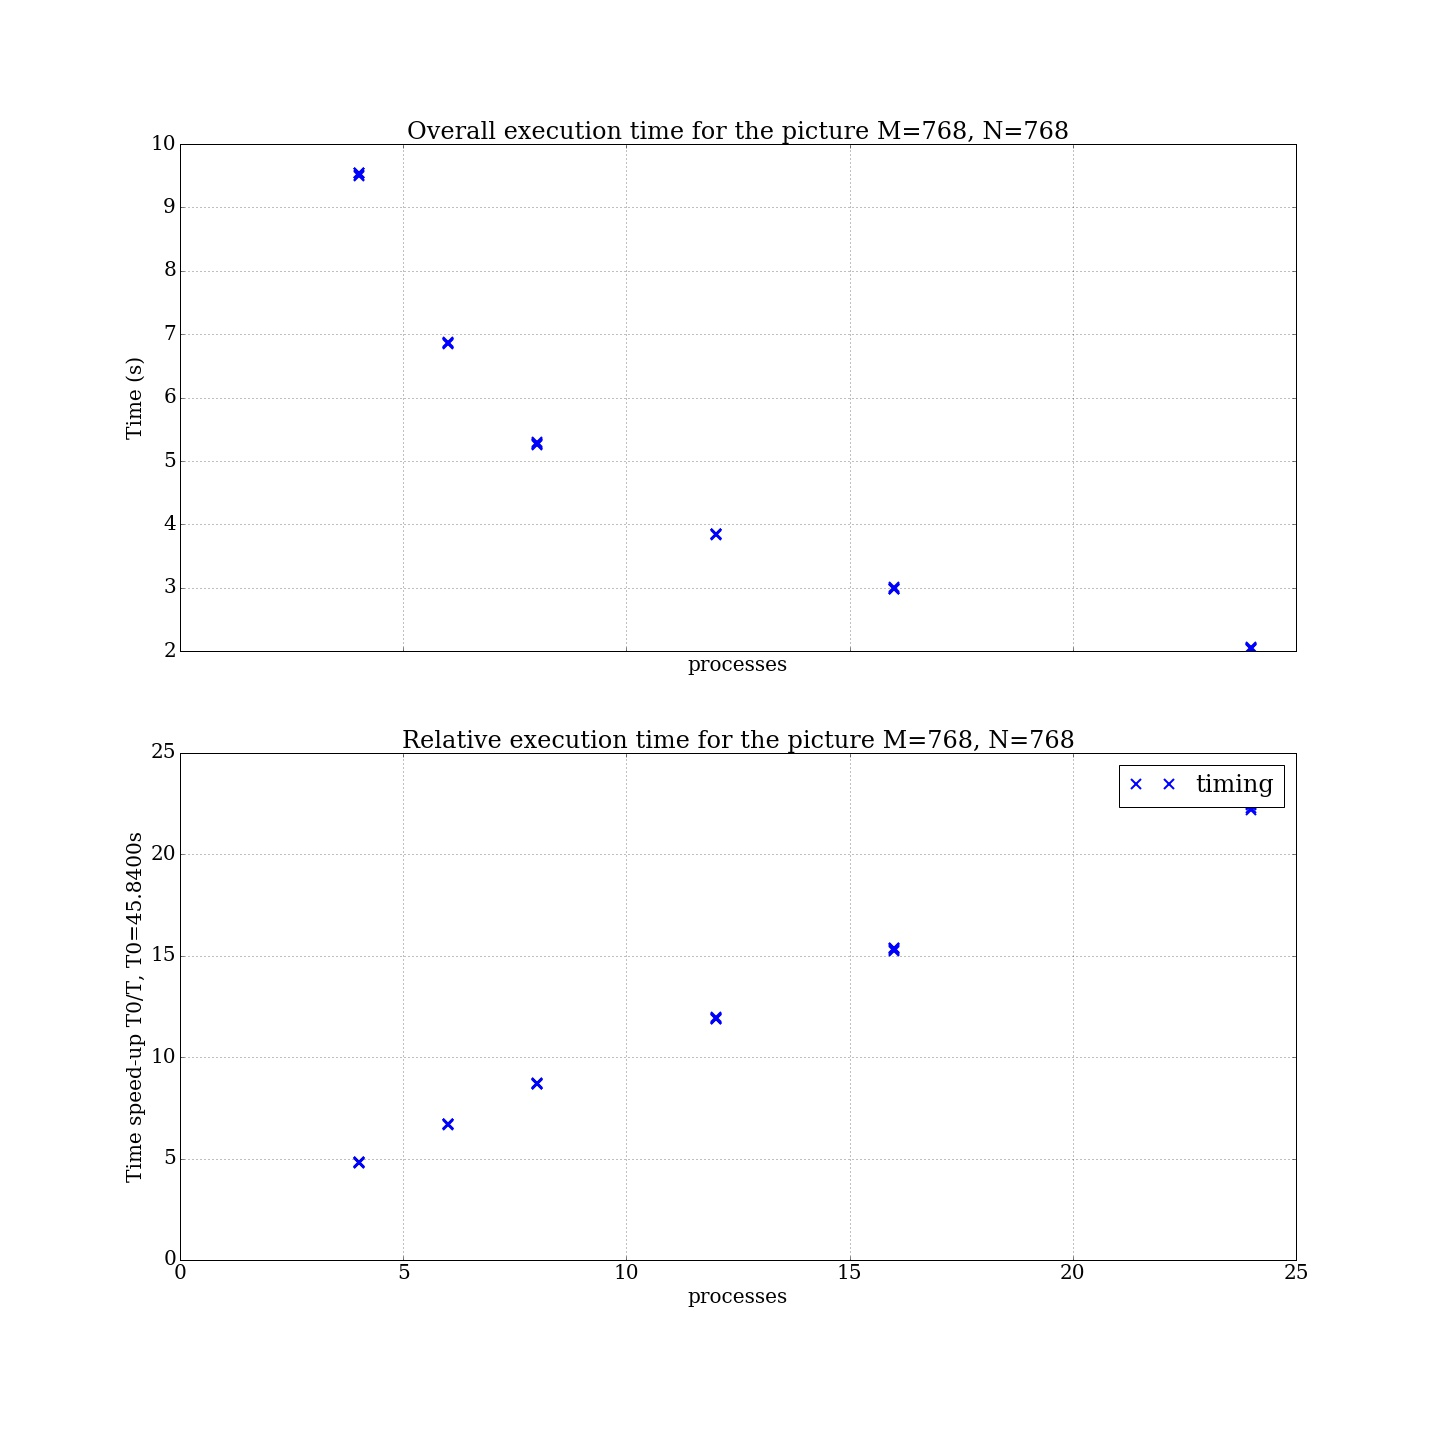
\includegraphics[scale=0.4]{exec_768x768.jpeg}
		\caption{Execution time and relative(to serial) execution time for the 768x768 pixel image.}\label{exec_4}
	\end{figure}

	\begin{figure}[H]	
		\centering
		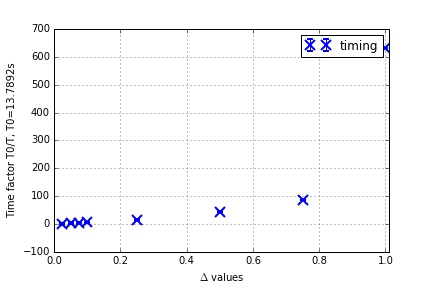
\includegraphics[scale=0.5]{itervs3.jpeg}
		\caption{Relative execution time for different values of $\Delta$. $T_0$ is at $\Delta=0.01$.}\label{iter3}
	\end{figure}

	
	\begin{figure}[H]	
		\centering
		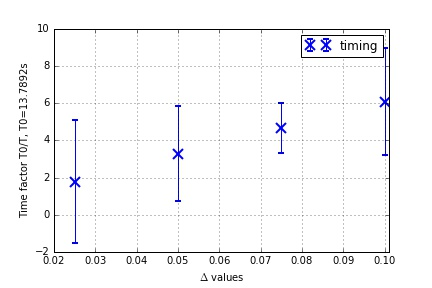
\includegraphics[scale=0.5]{itervs32.jpeg}
		\caption{Close-up for the relative execution time vs $\Delta$ values.}\label{iter32}
	\end{figure}

	
	\begin{figure}[H]	
		\centering
		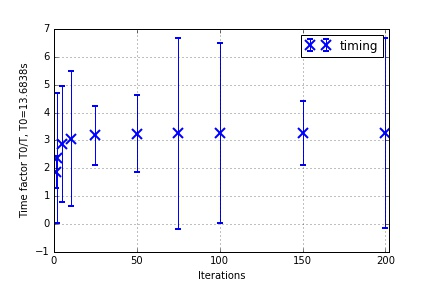
\includegraphics[scale=0.5]{itervs4.jpeg}
		\caption{Relative execution time for different intervals at which $\Delta$ was measured. $T_0$ for no measurement.}\label{iter4}
	\end{figure}

	
	\begin{figure}[H]	
		\centering
		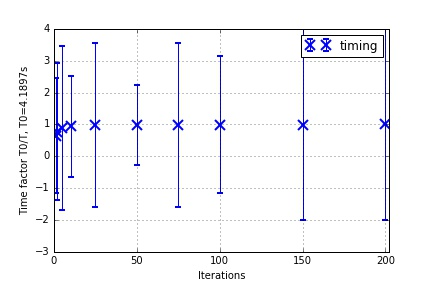
\includegraphics[scale=0.5]{itervs5.jpeg}
		\caption{Relative execution time for different intervals at which the average was measured. $T_0$ for no measurement.}\label{iter5}
	\end{figure}

	
	\begin{figure}[H]	
		\centering
		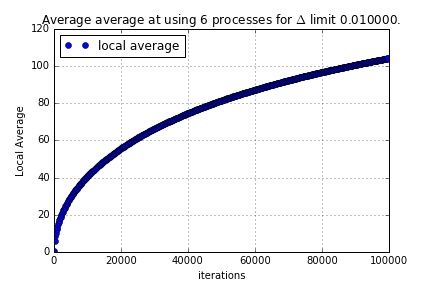
\includegraphics[scale=0.5]{local_avg_6_010000.jpeg}
		\caption{Average value of image pixel over 100,000 iteration for $\Delta=0.01$.}\label{avg1}
	\end{figure}

	
	\begin{figure}[H]	
		\centering
		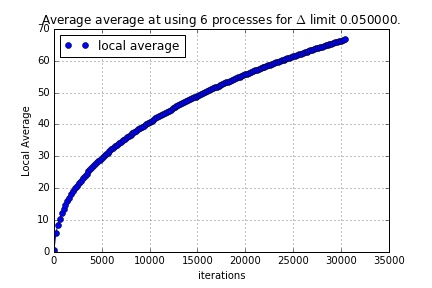
\includegraphics[scale=0.5]{local_avg_6_050000.jpeg}
		\caption{Average value of image pixel over 100,000 iteration for $\Delta=0.05$.}\label{avg2}
	\end{figure}

	
	\begin{figure}[H]	
		\centering
		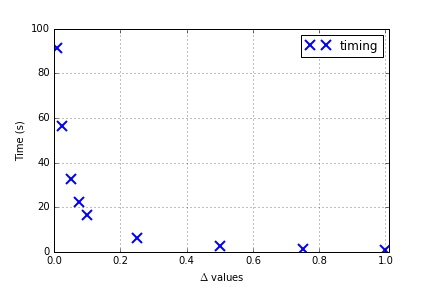
\includegraphics[scale=0.5]{serialvs3.jpeg}
		\caption{Execution time for the serial code for different values of $\Delta$.}\label{serial3}
	\end{figure}

	\begin{figure}[H]	
		\centering
		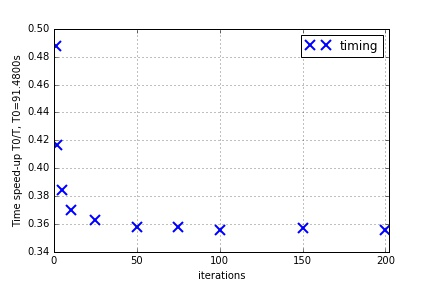
\includegraphics[scale=0.5]{serialvs4.jpeg}
		\caption{Relative execution time for different intervals at which $\Delta$ was measured. $T_0$ for no measurement.}\label{serial4}
	\end{figure}
	
	\begin{figure}[H]	
		\centering
		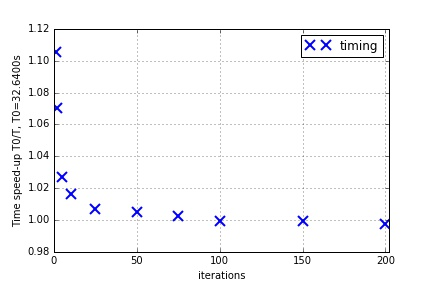
\includegraphics[scale=0.5]{serialvs5.jpeg}
		\caption{Relative execution time for different intervals at which the average was measured. $T_0$ for no measurement.}\label{serial5}
	\end{figure}

	\pagebreak
	\section{Appendix A - Pictures}
	
	\begin{figure}[H]	
		\centering
		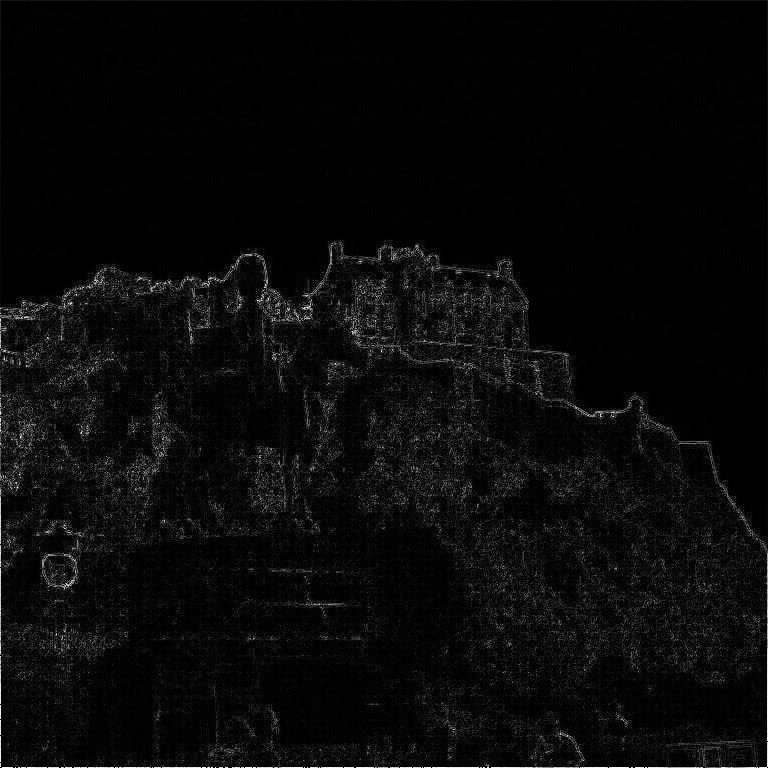
\includegraphics[scale=0.23]{edge768x768.jpg}
		\caption{Unprocessed image.}\label{pic0}
	\end{figure}
	
	\begin{figure}[H]	
		\centering
		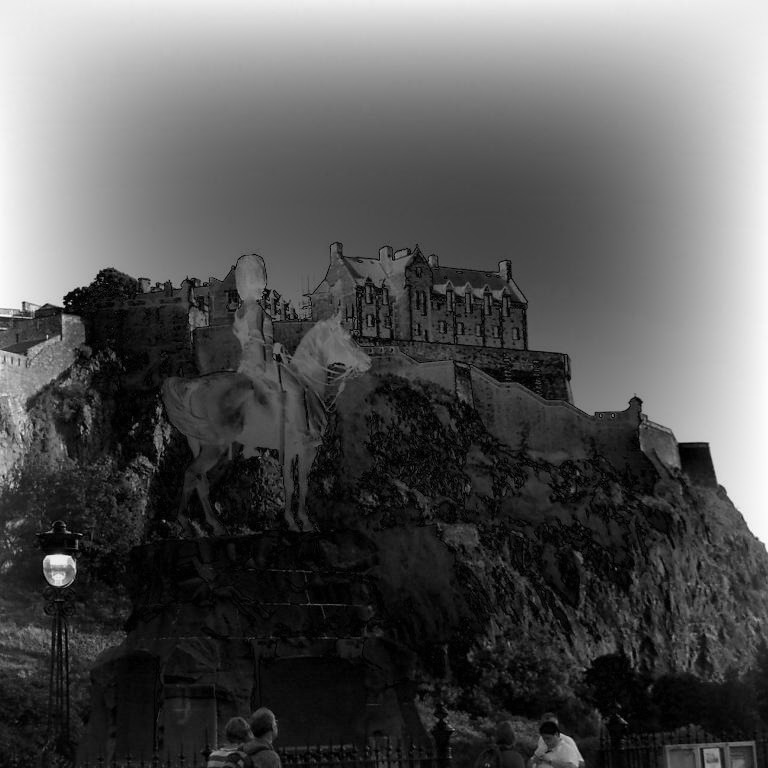
\includegraphics[scale=0.23]{edge768x768_050.jpg}
		\caption{Processed image with $\Delta=0.05$.}\label{pic5}
	\end{figure}

	\begin{figure}[H]	
		\centering
		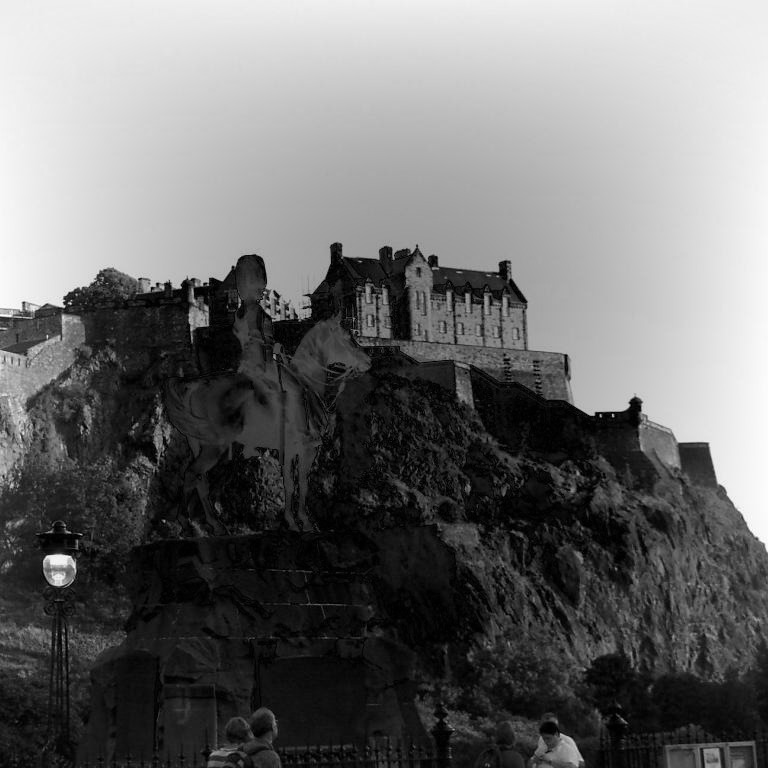
\includegraphics[scale=0.23]{edge768x768_010.jpg}
		\caption{Processed image with $\Delta=0.01$.}\label{pic1}
	\end{figure}

	\pagebreak
	
	\section{Appendix B - Serial Code}
	\begin{lstlisting}
	#include <stdio.h>
	#include <stdlib.h>
	#include <math.h>
	#include <string.h>
	#include <time.h>
	
	#include "pgmio.h"
	
	double average(double *times, int r, int iter);
	double mySum(void *myArray, int size);
	double myAverage(void *myArray, int size);
	float maxValue(float *myArray, int size);
	double avg_time(double *myArray, int size);
	float** make_2d_dyn(int rows, int cols);
	
	#define MAXITER 5000
	
	int main(int argc, char** argv)
	{
	/*
	The main part of the serial code. It executes the conversion of the pictures
	with just edges defined to the mode detailed picture. It uses just a single
	route (process) to achieve this goal.
	*/
	int i,j,iter=0;
	int rank=0, size=0;
	float local_sum, local_avg;
	char *ptr;
	double times[MAXITER];
	
	// set defaults, in case inputs are not given.
	int M=256, N=192, DELTA_FREQ=100, AVG_FREQ=200;
	float MAX_DELTA=0.05;
	int var_array[10] = {1, 2, 5, 10, 25, 50, 75, 100, 150, 200};
	float m_delta[9]  = {1., 0.75, 0.5, 0.25, 0.1, 0.075, 0.05, 0.025, 0.01};
	//read the inputs
	for (int arg = 0; arg < argc; arg++)
	{
	if (strcmp(argv[arg], "M") == 0)
	{
	M = (int)strtol(argv[arg+1], &ptr, 10);
	} else if (strcmp(argv[arg], "N") == 0)
	{
	N = (int)strtol(argv[arg+1], &ptr, 10);
	} else if (strcmp(argv[arg], "Df") == 0)
	{
	DELTA_FREQ = var_array[(int)strtol(argv[arg+1], &ptr, 10)-1];
	} else if (strcmp(argv[arg], "Af") == 0)
	{
	AVG_FREQ = var_array[(int)strtol(argv[arg+1], &ptr, 10)-1];
	} else if (strcmp(argv[arg], "MD") == 0)
	{
	MAX_DELTA = m_delta[(int)strtol(argv[arg+1], &ptr, 10)-1];
	}
	}
	
	//create the arrays which will be used for image processing
	float max_delta = MAX_DELTA + 1;
	float **masterbuf = make_2d_dyn(M, N);
	float **edge = make_2d_dyn(M+2, N+2);
	float **old = make_2d_dyn(M+2, N+2);
	float **new = make_2d_dyn(M+2, N+2);
	float **delta = make_2d_dyn(M, N);
	fflush(stdout);
	
	//start measuring the time & create the files to be read & written to
	clock_t start_time = clock();
	char filename[16], filename_end[22];
	sprintf(filename, "edge%dx%d.pgm", M, N);
	sprintf(filename_end, "edge%dx%d_%.3f.pgm", M, N, MAX_DELTA);
	
	printf("Reading %s\n", filename);
	pgmread(filename, *masterbuf, M, N);
	printf("Finished reading\n");
	
	//print statement used for post-processing
	printf("init size=-1 MP=-1 NP=-1 M=%d N=%d max_delta=%f delta_freq=%d avg_freq=%d\n", M, N, MAX_DELTA, DELTA_FREQ, AVG_FREQ);
	
	//fill the initial arrays with the edge values & the actual values from the
	// picture
	for (int i=0; i<M+2; i++)
	{
	for (int j=0; j<N+2; j++)
	{
	edge[i][j] = 255.0;
	}
	}
	for (i=1; i<M+1; i++)
	{
	for (j=1; j<N+1; j++)
	{
	edge[i][j] = masterbuf[i-1][j-1];
	}
	}
	
	for (int i=0; i<M+2; i++)
	{
	for (int j = 0; j < N+2; j++)
	{
	old[i][j] = edge[i][j];
	}
	}
	
	// start the main loop. Iterate over either the maximum number MAXITER
	// or until the maximum change (max_delta) is smaller than the threashold
	while (iter < MAXITER && MAX_DELTA < max_delta)
	{
	times[iter] = clock();
	// calculate the new values based on the old ones
	for (int i=1; i<M+1; i++)
	{
	for (int j=1; j<N+1; j++)
	{
	new[i][j] =  (old[i-1][j] + old[i+1][j] + old[i][j-1] + old[i][j+1] - edge[i][j]) * 0.25;
	}
	}
	
	// Calculate the maximum DELTA here
	if (iter % DELTA_FREQ == 0)
	{
	for (int i=0; i<M; i++)
	{
	for (int j=0; j<N; j++)
	{
	delta[i][j] = fabsf(old[i+1][j+1] - new[i+1][j+1]);
	}
	}
	max_delta = maxValue(*delta, M*N);
	printf("max_delta=%.10f iter=%d rank=%d size=%d limit_delta=%f\n", max_delta, iter, rank, size, MAX_DELTA);
	}
	
	// Calculate the average here
	if (iter % AVG_FREQ == 0)
	{
	local_avg = myAverage(*new, (M+2) * (N+2));
	printf("local_avg=%.10f iter=%d size=%d limit_delta=%f\n", local_avg, iter, size, MAX_DELTA);
	}
	
	// reassign the new values to the old so the iteration can restart
	for (int i=1; i<M+1; i++)
	{
	for (int j=1; j<N+1; j++)
	{
	old[i][j] = new[i][j];
	}
	}
	
	iter++;
	times[iter-1] -= clock();
	}
	
	//write the final values to the masterbuf
	for (int i=0; i<M; i++)
	{
	for (int j=0; j<N; j++)
	{
	masterbuf[i][j] = old[i+1][j+1];
	}
	}
	
	//write the latest values generated to the file
	printf("Writing\n");
	pgmwrite(filename_end, *masterbuf, M, N);
	printf("Finished writing\n");
	
	clock_t end_time = clock();
	
	// print values of the time for performance
	printf("iter=%d overall_time=%f iter_time=%f total_loop=%f max_delta=%f\n", iter, (double)(end_time-start_time)/(double)CLOCKS_PER_SEC, avg_time(times, iter), avg_time(times, iter) * iter, max_delta);
	
	// free the memory
	free(masterbuf);
	free(edge);
	free(old);
	free(new);
	free(delta);
	}
	
	
	// ---------------------------
	// Additional functions
	// ---------------------------
	
	float** make_2d_dyn(int rows, int cols)
	{
	/*
	Function that makes the dynamic allocation of memory for a 2D array of
	M rows & N columns.
	*/
	float **myArray = (float **) malloc(rows * sizeof(float *));
	myArray[0] = (float *) malloc(rows * cols * sizeof(float));
	for (int i = 1; i<rows; i++)
	myArray[i] = myArray[0] + i * cols;
	return myArray;
	}
	
	double mySum(void *myArray, int size)
	{
	/*
	Function that calculates the sum of an array of a given size.
	*/
	double sum = 0;
	float *x = (float *)myArray;
	for (int i = 0; i<size; i++)
	{
	sum += x[i];
	}
	return sum;
	}
	
	double myAverage(void *myArray, int size)
	{
	// Function that calculates the average of an array of a given size
	return mySum(myArray, size)/ (double)size;
	}
	
	float maxValue(float *myArray, int size)
	{
	// Function that calculates the maximum value from an array.
	int i;
	float max = 0;
	for (i = 0; i<size; i++)
	{
	if (max < myArray[i]) max = myArray[i];
	}
	return max;
	}
	
	double avg_time(double *myArray, int size)
	{
	/*
	Function that calculates the average time for an iteration. Different from
	myAverage & mySum because a different type of array was given.
	*/
	
	double sum = 0;
	double *x = (double *)myArray;
	for (int i=0; i<size; i++)
	{
	sum += x[i];
	}
	sum = sum / (double)size;
	return sum;
	}
	\end{lstlisting}
	\pagebreak
	
	\section{Appendix C - 2D Parallel Code}
	The main code for the 2d Parallel C code using MPI implementation: 
	\begin{lstlisting}
	#include <stdio.h>
	#include <stdlib.h>
	#include <math.h>
	#include <string.h>
	#include <mpi.h>
	
	#include "pgmio.h"
	#include "comms.h"
	#include "do_2d.h"
	
	#define MAXITER 100000
	double times[MAXITER];
	
	int main(int argc, char** argv)
	{
	int MN[2];
	int MP, NP;
	int i,j;
	int iter=0;
	int size, rank, left, right, up, down, MP_fact;
	float local_sum, global_sum, local_avg, global_avg;
	double start_time, make_MP_time, choose_neighbours, make_buff, reconstruct_time, barrier_time;
	char *ptr;
	
	MPI_Comm comm;
	MPI_Status status;
	
	// set defaults, in case inputs are not given.
	int M=768, N=768, DELTA_FREQ=100, AVG_FREQ=200;
	float MAX_DELTA=0.05;
	int val_array[10] = {1, 2, 5, 10, 25, 50, 75, 100, 150, 200};
	float m_delta[9] = {1., 0.75, 0.5, 0.25, 0.1, 0.075, 0.05, 0.025, 0.01};
	//read the inputs
	for (int arg = 0; arg < argc; arg++)
	{
	if (strcmp(argv[arg], "M") == 0)
	{
	M = (int)strtol(argv[arg+1], &ptr, 10);
	} else if (strcmp(argv[arg], "N") == 0)
	{
	N = (int)strtol(argv[arg+1], &ptr, 10);
	} else if (strcmp(argv[arg], "Df") == 0)
	{
	DELTA_FREQ = val_array[(int)strtol(argv[arg+1], &ptr, 10)-1];
	} else if (strcmp(argv[arg], "Af") == 0)
	{
	AVG_FREQ = val_array[(int)strtol(argv[arg+1], &ptr, 10)-1];
	} else if (strcmp(argv[arg], "MD") == 0)
	{
	MAX_DELTA = m_delta[(int)strtol(argv[arg+1], &ptr, 10)-1];
	}
	}
	
	//create the arrays which will be used for image processing
	float max_delta = MAX_DELTA + 1;
	float masterbuf[M][N];
	fflush(stdout);
	
	//generate the name of the files to be read & written to
	char filename[16], filename_end[22];
	sprintf(filename, "edge%dx%d.pgm", M, N);
	sprintf(filename_end, "edge%dx%d_%.3f.pgm", M, N, MAX_DELTA);
	
	//read the initial data
	printf("Reading\n");
	pgmread(filename, masterbuf, M, N);
	printf("Finished reading\n");
	
	
	// MPI STARTS FROM HERE
	comm = MPI_COMM_WORLD;
	
	MPI_Init(NULL,NULL);
	MPI_Comm_rank(comm, &rank);
	MPI_Comm_size(comm, &size);
	
	start_time = -MPI_Wtime(); //timing the entire MPI section
	
	// choosing the optimum split for the big array
	make_MP_time = -MPI_Wtime();
	choose_MN(MN, size, M, N);
	MP = MN[0];
	NP = MN[1];
	make_MP_time += MPI_Wtime();
	
	// create the smaller arrays
	float max_delta_thread[size];
	float buf[MP][NP];
	float edge[MP+2][NP+2];
	float old[MP+2][NP+2];
	float new[MP+2][NP+2];
	float delta[MP*NP];
	
	// map the neighbours based on current rank, left righ up & down
	choose_neighbours = -MPI_Wtime();
	MP_fact = M / MP;
	right = rank + 1;
	left = rank - 1;
	up = rank - MP_fact;
	down = rank + MP_fact;
	if (rank % MP_fact== 0)
	{
	left = MPI_PROC_NULL;
	}
	if ((rank + 1) % MP_fact == 0)
	{
	right = MPI_PROC_NULL;
	}
	if (down >= size)
	{
	down = MPI_PROC_NULL;
	}
	if (up < 0)
	{
	up = MPI_PROC_NULL;
	}
	choose_neighbours += MPI_Wtime();
	
	// initial print detailing all the current variables. To be used in post processing
	if (rank==0) printf("init size=%d MP=%d NP=%d M=%d N=%d max_delta=%f delta_freq=%d avg_freq=%d\n", size, MP, NP, M, N, MAX_DELTA, DELTA_FREQ, AVG_FREQ);
	
	// Scatter data and assign proper values to corresponding arrays
	make_buff = -MPI_Wtime();
	my_Scatter(buf, M, N, masterbuf, rank, MP, NP); // scatter the value to appropriate buf according to the rank
	
	for (int i=0; i<MP+2; i++)
	{
	for (int j=0; j<NP+2; j++)
	{
	edge[i][j] = 255; // the edge matrix is given 255, including the halo
	old[i][j] = 255; // same for the old matrix
	}
	}
	for (i=1; i<MP+1; i++)
	{
	for (j=1; j<NP+1; j++)
	{
	edge[i][j] = buf[i-1][j-1]; // edge matrix will record the just the intial edge picture
	old[i][j] = buf[i-1][j-1]; // old initially looks like the edge, as it is the initial iteration
	}
	}
	make_buff += MPI_Wtime();
	
	// start the main loop
	// loop finishes when either the maximum number of iterations has been achieved
	// or the maximum change in a pixel past which it becomes redundent is computed.
	// if no max_delta, we just go to max iterations.
	while (iter < MAXITER && MAX_DELTA < max_delta)
	{
	times[iter] = -MPI_Wtime(); // record the time for each loop
	
	// send the halos to the corresponding neighbours
	communicate_lr(old, left, right, MP, NP);
	communicate_ud(old, up, down, MP, NP);
	
	// compute the new pixel value here
	for (int i=1; i<MP+1; i++)
	{
	for (int j=1; j<NP+1; j++)
	{
	new[i][j] =  (old[i-1][j] + old[i+1][j] + old[i][j-1] + old[i][j+1] - edge[i][j]) * 0.25;
	}
	}
	
	// compute the value of the maximum delta change after a certain number of iterations
	if (iter % DELTA_FREQ == 0)
	{
	for (int i=0; i<MP; i++)
	{
	for (int j=0; j<NP; j++)
	{
	delta[i*NP+j] = fabsf(old[i+1][j+1] - new[i+1][j+1]); // for the current rank
	}
	}
	// after all ranks calculated their change, from each array, the maximum will be send to another array that hold just the maximum value
	MPI_Allreduce(delta, max_delta_thread, size, MPI_FLOAT, MPI_MAX, comm);
	max_delta = maxValue(max_delta_thread, size); //get the new maximum for the entire picture
	if (rank==0) printf("max_delta=%.10f iter=%d rank=%d size=%d limit_delta=%f\n", max_delta, iter, rank, size, MAX_DELTA); // for post processing
	}
	
	// Calculate the average pixel value
	if (iter % AVG_FREQ == 0)
	{
	// get the local average and the local sum
	local_avg = myAverage(buf, MP * NP);
	local_sum = mySum(buf, MP * NP);
	MPI_Reduce(&local_sum, &global_sum, 1, MPI_FLOAT, MPI_SUM, 0, comm); // send the local sum to a global sum stored in MASTER
	if (rank == 0)
	{
	// the MASTER now calculates the actual global average prints it for post processing.
	global_avg = global_sum / (double)(M * N);
	printf("local_avg=%.10f iter=%d size=%d limit_delta=%f\n", global_avg, iter, size, MAX_DELTA);
	}
	}
	
	// the new becomes the old for the next iteration & the cycle begins again
	for (int i=1; i<MP+1; i++)
	{
	for (int j=1; j<NP+1; j++)
	{
	old[i][j] = new[i][j];
	buf[i-1][j-1] = old[i][j];
	}
	}
	
	times[iter] += MPI_Wtime();
	iter++;
	}
	
	// star reconstructing the MASTERBUF mastrix & time everything
	reconstruct_time = -MPI_Wtime();
	my_Gather(masterbuf, MP, NP, buf, rank, size, M, N);
	reconstruct_time += MPI_Wtime();
	barrier_time = -MPI_Wtime();
	MPI_Barrier(comm); // wait for all processes to send their buf
	barrier_time += MPI_Wtime();
	
	// calculate the current value of the global sum & average
	local_sum = mySum(buf, MP * NP);
	MPI_Reduce(&local_sum, &global_sum, 1, MPI_FLOAT, MPI_SUM, 0, comm);
	
	// print all the times for each process for post processing
	printf("avg_time=%.10f rank=%d overall_time=%.10f total_loop=%.10f make_MP_time=%.10f choose_neighbours=%.10f make_buff=%.10f reconstruct_time=%.10f barrier_time=%.10f\n",
	avg_time(times, iter), rank, start_time+MPI_Wtime(), avg_time(times, iter) * iter, make_MP_time, choose_neighbours, make_buff, reconstruct_time, barrier_time);
	
	// if rank is MASTER, then print the global avg, max_delta achieved & the iteration at which the loop stopped
	// also, write the final picture back to memory
	if (rank == 0)
	{
	global_avg = global_sum / (double)(M * N);
	printf("global_avg=%.10f max_delta=%.10f iter=%d\n", global_avg, max_delta, iter);
	printf("Writing\n");
	pgmwrite(filename_end, masterbuf, M, N);
	printf("Finished writing\n");
	}
	
	// finalise the MPI
	MPI_Barrier(comm);
	MPI_Finalize();
	}
	
	
	// ---------------------------
	// Additional functions
	// ---------------------------
	
	
	void choose_MN(void *myArray, int size, int M, int N)
	{
	/*
	Function that calculates the the optimum MP & NP based on the number of
	processes acting. The basic concept is to find the closest 2 integers
	that multiplied equal to size. It then return an array to be allocated
	to MP & NP.
	*/
	int M_i, N_i;
	int MP, NP;
	int *MN = (int *)myArray;
	int done_choosing_MN = 0, cont = 1;
	
	if (fmod(size, sqrt(size)) == 0)
	{
	// is square of another number
	MN[0] = M / (int)sqrt(size);
	MN[1] = N / (int)sqrt(size);
	}
	else
	{
	// start mapping the 2 closest intergers that multiply give P
	while (done_choosing_MN == 0)
	{
	M_i = size / sqrt(size) + cont;
	while(size % M_i != 0)
	{
	cont++;
	M_i = size / sqrt(size) + cont;
	}
	N_i = size / M_i;
	cont++; //if they divide, but not divide in the next if, this must be increased so you actually get the next number
	
	if (N_i == 1)
	{
	// N_i will go down as M_i is increased, so we might reach the end here
	if (M % M_i == 0)
	{
	// see if we actually divide this part, otherwise go to the next axis and divide that
	MN[0] = M / M_i;
	MN[1] = N;
	}
	else
	{
	MN[0] = M;
	MN[1] = N / M_i;
	}
	done_choosing_MN = 1; // we are actually done choosing now
	}
	else if(fmod(M, M_i) == 0 && fmod(N, N_i) == 0)
	{ //if the numbers are not 0 and they both divide these axis, we will chose these ones, if not, we will swap the division,
	MN[0] = M / M_i;
	MN[1] = N / N_i;
	done_choosing_MN = 1;
	}
	else if (fmod(M, N_i) == 0 && fmod(N, M_i) == 0)
	{
	MN[0] = M / N_i;
	MN[1] = N / M_i;
	done_choosing_MN = 1;
	}
	}
	}
	}
	
	void my_Scatter(void *buf, int M, int N, float masterbuf[M][N], int rank, int MP, int NP)
	{
	/*
	Function to scatter the data between processes from the initial buffer based
	on the current proces rank.
	*/
	int i, j;
	int x, y, chunks;
	float *lbuf = (float *)buf;
	
	chunks = M / MP;
	x = rank % chunks;
	y = rank / chunks;
	
	for (i=0; i<MP; i++)
	{
	for (j=0; j<NP; j++)
	{
	lbuf[i*NP+j] = masterbuf[x*MP+i][y*NP+j];
	}
	}
	}
	
	
	void my_Gather(void *masterbuf, int MP, int NP, float buf[MP][NP], int rank, int size, int M, int N)
	{ //I'm making my own Gather, with blackjack & hookers
	/*
	Function that does the MPI_GATHER but for the 2D case.
	It takes the the buff of each thread going in and sending to MASTER then wait
	for completion. MASTER will write its own buff to masterbuf, then start
	to receive stuff from other processes in order & writing them accordingly.
	*/
	int i, j, k;
	int x, y, chunks;
	float *lmbuf = (float *)masterbuf;
	chunks = M / MP;
	float localbuf[MP][NP];
	
	if (rank != 0)
	{ //if not the MASTER, send the buff
	communicate_chunk(buf, rank, 0, MP, NP);
	}
	else
	{
	my_Gather_process(lmbuf, MP, NP, buf, rank, M, N); // write the initial buff
	for (k=1; k<size; k++)
	{ // start to write the other buffs to the main one
	communicate_chunk(localbuf, 0, k, MP, NP);
	my_Gather_process(lmbuf, MP, NP, localbuf, k, M, N);
	}
	}
	}
	
	void my_Gather_process(float *lmbuf, int MP, int NP, float buf[MP][NP], int rank, int M, int N)
	{ //I'm making my own Gather, with blackjack & hookers
	/*
	Second part of gathering. This function actually writes the data to the master buff.
	Takes the buff & the masterbuf and writes the buff into the master.
	*/
	int i, j;
	int x, y, chunks;
	fflush(stdout);
	chunks = M / MP;
	
	x = rank % chunks;
	y = rank / chunks;
	fflush(stdout);
	
	for (i=0; i<MP; i++)
	{
	for (j=0; j<NP; j++)
	{
	lmbuf[(x*MP+i)*N+y*NP+j] = buf[i][j];
	fflush(stdout);
	}
	}
	}
	
	double mySum(void *myArray, int size)
	{
	/*
	Function that calculates the sum of an array of a given size.
	*/
	double sum = 0;
	float *x = (float *)myArray;
	for (int i = 0; i<size; i++)
	{
	sum += x[i];
	}
	return sum;
	}
	
	double myAverage(void *myArray, int size)
	{
	// Function that calculates the average of an array of a given size
	return mySum(myArray, size)/ (double)size;
	}
	
	float maxValue(float *myArray, int size)
	{
	// Function that calculates the maximum value from an array.
	int i;
	float max = 0;
	for (i = 0; i<size; i++)
	{
	if (max < myArray[i]) max = myArray[i];
	}
	return max;
	}
	
	double avg_time(double *myArray, int size)
	{
	/*
	Function that calculates the average time for an iteration. Different from
	myAverage & mySum because a different type of array was given.
	*/
	
	double sum = 0;
	double *x = (double *)myArray;
	for (int i=0; i<size; i++)
	{
	sum += x[i];
	}
	sum = sum / (double)size;
	return sum;
	}
	\end{lstlisting}
	
	Alongside this code, a header file is used for all the functions present in this file:
	\begin{lstlisting}
	void choose_MN(void *myArray, int size, int M, int N);
	void my_Scatter(void *buf, int M, int N, float masterbuf[M][N], int rank, int MP, int NP);
	void my_Gather(void *masterbuf, int MP, int NP, float buf[MP][NP], int rank, int size, int M, int N);
	void my_Gather_process(float *lmbuf, int MP, int NP, float buf[MP][NP], int rank, int M, int N);
	double mySum(void *myArray, int size);
	double myAverage(void *myArray, int size);
	float maxValue(float *myArray, int size);
	double avg_time(double *myArray, int size);
	\end{lstlisting}
	\pagebreak
	
	\section{Appendix D - Comms and pgmio Code}
	\subsection{Comms.c}
	In order to achieve proper communication, \textbf{comms.c} was created. It uses MPI send and recv protocols to send and received data between processes.
	\begin{lstlisting}
	#include <stdio.h>
	#include <stdlib.h>
	#include <math.h>
	#include <string.h>
	#include <mpi.h>
	
	
	void communicate_lr(void *oldbuf, int left, int right, int MP, int NP)
	{
	/*
	Function that makes the communication to the left and right neighbours.
	It takes the buf, the left & right neightbours. Then sends the appropriate
	values to them. In this case, the 2nd column to left & the second to last column to right.
	Then it receives from the the halo values.
	*/
	float *buf = (float *)oldbuf;
	int prev = left;
	int next = right;
	MPI_Status status_p;
	MPI_Request request_p;
	MPI_Status status_n;
	MPI_Request request_n;
	
	MPI_Issend(&buf[(NP+2)*MP+1], NP, MPI_FLOAT, next, 0, MPI_COMM_WORLD, &request_p);
	MPI_Issend(&buf[(NP+2)+1], NP, MPI_FLOAT, prev, 0, MPI_COMM_WORLD, &request_n);
	MPI_Recv(&buf[1], NP, MPI_FLOAT, prev, 0, MPI_COMM_WORLD, &status_p);
	MPI_Recv(&buf[(NP+2)*(MP+1)+1], NP, MPI_FLOAT, next, 0, MPI_COMM_WORLD, &status_n);
	
	MPI_Wait(&request_p, &status_p);
	MPI_Wait(&request_n, &status_n);
	}
	
	void communicate_ud(void *oldbuf, int up, int down, int MP, int NP)
	{
	/*
	Function that sends & receives the halos from the neighbours positioned
	above and below the current process in the topology.
	This function uses the Type_vector MPI method to actually map the values
	needed to be sent.
	*/
	float *buf = (float *) oldbuf;
	int prev = up;
	int next = down;
	MPI_Status status_p;
	MPI_Request request_p;
	MPI_Status status_n;
	MPI_Request request_n;
	
	MPI_Datatype new_array;
	
	MPI_Type_vector(MP, 1, NP+2, MPI_FLOAT, &new_array);
	MPI_Type_commit(&new_array);
	
	MPI_Issend(&buf[(NP+2)+1], 1, new_array, up, 0, MPI_COMM_WORLD, &request_p);
	MPI_Issend(&buf[(NP+2)+NP], 1, new_array, down, 0, MPI_COMM_WORLD, &request_n);
	MPI_Recv(&buf[NP+2], 1, new_array, up, 0, MPI_COMM_WORLD, &status_p);
	MPI_Recv(&buf[(NP+2)+NP+1], 1, new_array, down, 0, MPI_COMM_WORLD, &status_n);
	
	MPI_Wait(&request_p, &status_p);
	MPI_Wait(&request_n, &status_n);
	}
	
	void communicate_chunk(void *buf, int rank, int recv_rank, int MP, int NP)
	{
	/*
	Function that send the entire buf to rank 0. MASTER then in turns receives
	the entire buf.
	*/
	MPI_Status status;
	MPI_Request request;
	float *buff =(float *)buf;
	if (rank!=0)
	{
	MPI_Send(&buff[0], MP*NP, MPI_FLOAT, recv_rank, 0, MPI_COMM_WORLD);
	}
	else
	{
	MPI_Recv(&buff[0], MP*NP, MPI_FLOAT, recv_rank, 0, MPI_COMM_WORLD, &status);
	}
	}
	\end{lstlisting}
	The appropriate header file for comms.c.
	\begin{lstlisting}
	void communicate_lr(void *oldbuf, int left, int right, int MP, int NP);
	void communicate_ud(void *oldbuf, int up, int down, int MP, int NP);
	void communicate_chunk(void *oldbuf, int rank, int recv_rank, int MP, int NP);
	\end{lstlisting}
	\subsection{pgmio.c}
	The pgmio.c file was provided for this assignment as an additional code for a Case study presented in the lectures. The code was created by the lecturer. The code was not created by the author of this report.
	\begin{lstlisting}
	/*
	* This file contains C routines for the MPI Casestudy.
	*
	* "pgmread" reads in a PGM picture and can be called as follows:
	*
	*    float buf[M][N];
	*    pgmread("edge.pgm", buf, M, N);
	*
	* "pgmwrite" writes an array as a PGM picture and can be called as follows:
	*
	*    float buf[M][N];
	*    pgmwrite("picture.pgm", buf, M, N);
	*
	* "pgmsize" returns the size of a PGM picture and can be called as follows:
	*
	*    int nx, ny;
	*    pgmsize("edge.pgm", &nx, &ny);
	*
	*  To access these routines, add the following to your program:
	*
	*    #include "pgmio.h"
	*
	*  Note: you MUST link with the maths library -lm to access fabs etc.
	*/
	
	
	#include <stdio.h>
	#include <stdlib.h>
	#include <math.h>
	
	#include "pgmio.h"
	
	#define MAXLINE 128
	
	/*
	*  Routine to get the size of a PGM data file
	*
	*  Note that this assumes a single line comment and no other white space.
	*/
	void datread(char *filename, void *vx, int nx, int ny)
	{
	FILE *fp;
	
	int nxt, nyt, i, j, t;
	
	float *x = (float *) vx;
	
	if (NULL == (fp = fopen(filename,"r")))
	{
	fprintf(stderr, "datread: cannot open <%s>\n", filename);
	exit(-1);
	}
	
	fscanf(fp,"%d %d",&nxt,&nyt);
	
	if (nx != nxt || ny != nyt)
	{
	fprintf(stderr,
	"datread: size mismatch, (nx,ny) = (%d,%d) expected (%d,%d)\n",
	nxt, nyt, nx, ny);
	exit(-1);
	}
	
	/*
	*  Must cope with the fact that the storage order of the data file
	*  is not the same as the storage of a C array, hence the pointer
	*  arithmetic to access x[i][j].
	*/
	
	for (j=0; j<ny; j++)
	{
	for (i=0; i<nx; i++)
	{
	fscanf(fp,"%d", &t);
	x[(ny-j-1)+ny*i] = t;
	}
	}
	
	fclose(fp);
	}
	
	void pgmsize(char *filename, int *nx, int *ny)
	{
	FILE *fp;
	
	char *cret;
	int iret;
	
	char dummy[MAXLINE];
	int n = MAXLINE;
	
	if (NULL == (fp = fopen(filename,"r")))
	{
	fprintf(stderr, "pgmsize: cannot open <%s>\n", filename);
	exit(-1);
	}
	
	cret = fgets(dummy, n, fp);
	cret = fgets(dummy, n, fp);
	
	iret = fscanf(fp,"%d %d", nx, ny);
	
	fclose(fp);
	}
	
	
	/*
	*  Routine to read a PGM data file into a 2D floating point array
	*  x[nx][ny]. Because of the way C handles (or fails to handle!)
	*  multi-dimensional arrays we have to cast the pointer to void.
	*
	*  Note that this assumes a single line comment and no other white space.
	*/
	
	void pgmread(char *filename, void *vx, int nx, int ny)
	{
	FILE *fp;
	
	int nxt, nyt, i, j, t;
	char dummy[MAXLINE];
	int n = MAXLINE;
	
	char *cret;
	int iret;
	
	float *x = (float *) vx;
	
	if (NULL == (fp = fopen(filename,"r")))
	{
	fprintf(stderr, "pgmread: cannot open <%s>\n", filename);
	exit(-1);
	}
	
	cret = fgets(dummy, n, fp);
	cret = fgets(dummy, n, fp);
	
	iret = fscanf(fp,"%d %d",&nxt,&nyt);
	
	if (nx != nxt || ny != nyt)
	{
	fprintf(stderr,
	"pgmread: size mismatch, (nx,ny) = (%d,%d) expected (%d,%d)\n",
	nxt, nyt, nx, ny);
	exit(-1);
	}
	
	iret = fscanf(fp,"%d",&i);
	
	/*
	*  Must cope with the fact that the storage order of the data file
	*  is not the same as the storage of a C array, hence the pointer
	*  arithmetic to access x[i][j].
	*/
	
	for (j=0; j<ny; j++)
	{
	for (i=0; i<nx; i++)
	{
	iret = fscanf(fp,"%d", &t);
	x[(ny-j-1)+ny*i] = t;
	}
	}
	
	fclose(fp);
	}
	
	
	/*
	*  Routine to write a PGM image file from a 2D floating point array
	*  x[nx][ny]. Because of the way C handles (or fails to handle!)
	*  multi-dimensional arrays we have to cast the pointer to void.
	*/
	
	void pgmwrite(char *filename, void *vx, int nx, int ny)
	{
	FILE *fp;
	
	int i, j, k, grey;
	
	float xmin, xmax, tmp, fval;
	float thresh = 255.0;
	
	float *x = (float *) vx;
	
	if (NULL == (fp = fopen(filename,"w")))
	{
	fprintf(stderr, "pgmwrite: cannot create <%s>\n", filename);
	exit(-1);
	}
	
	printf("Writing %d x %d picture into file: %s\n", nx, ny, filename);
	
	/*
	*  Find the max and min absolute values of the array
	*/
	
	xmin = fabs(x[0]);
	xmax = fabs(x[0]);
	
	for (i=0; i < nx*ny; i++)
	{
	if (fabs(x[i]) < xmin) xmin = fabs(x[i]);
	if (fabs(x[i]) > xmax) xmax = fabs(x[i]);
	}
	
	if (xmin == xmax) xmin = xmax-1.0;
	
	fprintf(fp, "P2\n");
	fprintf(fp, "# Written by pgmio::pgmwrite\n");
	fprintf(fp, "%d %d\n", nx, ny);
	fprintf(fp, "%d\n", (int) thresh);
	
	k = 0;
	
	for (j=ny-1; j >=0 ; j--)
	{
	for (i=0; i < nx; i++)
	{
	/*
	*  Access the value of x[i][j]
	*/
	
	tmp = x[j+ny*i];
	
	/*
	*  Scale the value appropriately so it lies between 0 and thresh
	*/
	
	fval = thresh*((fabs(tmp)-xmin)/(xmax-xmin))+0.5;
	grey = (int) fval;
	
	fprintf(fp, "%3d ", grey);
	
	if (0 == (k+1)%16) fprintf(fp, "\n");
	
	k++;
	}
	}
	
	if (0 != k%16) fprintf(fp, "\n");
	fclose(fp);
	}
	
	\end{lstlisting}
	The additional header file for pgmio code. 
	\begin{lstlisting}
	void datread(char *filename, void *vx, int nx, int ny);
	void pgmread(char *filename, void *vx, int nx, int ny);
	void pgmwrite(char *filename, void *vx, int nx, int ny);
	\end{lstlisting}
	
	\section{Appendix E - Makefile and PBS file}
	\subsection{Makefile}
	The following is an additional file enabling an easy compilation of the 2d Parallel Code (\textit{do\_2d.c}. For the serial case, \textit{do\_2d.c} is replaced by \textit{do\_serial.c} or however the user chooses to name the file. Once the Makefile was created, in \textit{Terminal}, the user can run \textbf{make} command, with all the appropriate files in the same folder to compile the code.
	
	\begin{lstlisting}
	
	CC=	mpicc
	LIB=	-lm
	
	#
	# Object files
	#
	OBJ=	do_2d.o \
	pgmio.o \
	comms.o
	
	
	#
	# Compile
	#
	do_2d:	$(OBJ)
	$(CC) -o $@ $(OBJ) $(LIB)
	
	.c.o:
	$(CC) -c $<
	
	#
	# Clean out object files and the executable.
	#
	clean:
	rm *.o do_2d
	\end{lstlisting}
	
	\subsection{PBS file}
	In order to run run this code, 2 options are possible. Firstly, the user can run in the command line the following command to execute the \textit{do\_2d.c} script, with some \textit{arguments} (see the beginning of the c code for arguments). The script runs 6 processes in this case.
	\begin{lstlisting}
	TMPDIR=/tmp mpirun -np 6 ./do_2d args
	\end{lstlisting}
	
	In addition, to run the code on ARCHER, for multiple values of a parameter (i) several times (j), the following PBS file can be submitted. The PBS file has to have the format: \textit{nameofcompiledCcode.pbs}.
	
	\begin{lstlisting}
	
	#PBS -A y14-CDT-Soton
	#PBS -j oe
	#PBS -l walltime=00:10:00
	#PBS -l select=1
	
	#----------------------------------------------------------#
	# You should only have to change the following single line #
	#----------------------------------------------------------#
	
	
	cd $PBS_O_WORKDIR
	
	OMPPROG=`basename $PBS_JOBNAME .pbs`
	
	echo '--------------------------------------------------------------------------------'
	
	echo 'Running OpenMP program' $OMPPROG 'on' $OMP_NUM_THREADS 'threads'
	
	echo 'Started at' `date`
	echo '--------------------------------------------------------------------------------'
	
	for j in (1..5)
	do
	for i in (1..10)
	(time aprun -n 6 ./$OMPPROG M 768 N 768 Df $i) 2>&1
	end
	end
	echo '--------------------------------------------------------------------------------'
	echo 'Finished at' `date`
	\end{lstlisting}
	\pagebreak
\end{document}